\chapter{identPy: a Software for Parameter Estimation}

\label{ch: software}

In order to estimate the parameters of mathematical models, such as the one presented on chapter \ref{ch: Mod}, a python library called \textit{identPy} was developed by the author. \textit{identPy} provides a customizable framework for parameter estimation with built-in mathematical models and estimation methods. 

With this tool, comparison between performance of methods and precision of models can be easily done. Also, users are allowed to customize or create new features to match their needs without having to rewrite the entire framework, reducing time spent on coding. A Graphical User Interface (GUI) was developed as well, providing a simple environment where users can apply the estimation tool without any contact with the code.

The entire library and GUI were written in Python 3, a powerful, simple and fast high-level programming language that has gained large space in various sectors of industry and academy. Its rise is due mainly to the enormous number of libraries and forums developed and maintained by the users. Some examples of libraries used in this project are \textit{numpy} (for scientific computing), \textit{matplotlib} (graph plotting) and \textit{PySide2} (GUI toolkit). Also, python is open-source, not requiring a paid software to code and most of its applications are free.

The following sections describe how the library is organized and illustrate the estimation process using \textit{identPy} GUI.

\section{\textit{identPy} Library}

\textit{identPy} was developed as a python library so users can simply install the package and apply its features as needed. The library, as well as related scripts and files, is hosted on a \href{https://github.com/gnegrelli/identPy}{GitHub repository} and maintained by the author.

The library contains four packages named \textbf{error}, \textbf{method}, \textbf{model} and \textbf{objects}. Each one of those packages initialize core python classes developed for this framework. The entire library was built using packages in order to allow future contributors to work on top of a basic architecture.

The \textbf{error} package comprises the methods used to evaluate the functional error $J(p)$. Currently, only weighted $l^{2}$-norm is implemented.

Inside \textbf{method} package, users will find the estimation methods implemented by the author and used on this study, as well as auxiliary scripts for parameter classification. A script containing a Particle Swarm Optimization algorithm implementation can be found in this package

All classes with mathematical models are organized inside the \textbf{model} package. Besides the WPP equivalent model presented before, this package contains simple models used for testing, such as Spring-Mass and Pendulum systems, and other complex models used in previous studies, such as Linearized Z-IM Load Model. It also contains a subpackage with implicit methods, such as the Runge-Kutta method, applied to obtain the behaviour of these models.

Finally, the estimator object and all abstract classes developed are organized inside \textbf{objects}. The Estimator object is responsible for building the estimation framework, by gathering the measured data, model and estimation methods, and executing it. The abstract classes located here constitute base objects from where the other classes can inherit.

\section{\textit{identPy} GUI}

The \textit{identPy} GUI was created with \textit{Qt}, a software for design of user interfaces and applications. The views and scripts created specifically for the GUI application are hosted on a different \href{https://github.com/gnegrelli/identPy_GUI}{repository}. When the application is launched, a starting window with information about the software is displayed, as shown in Figure \ref{fig: initial_page}.

\begin{figure}[h]
	\caption{Representation of software starting view}
	\begin{center}
		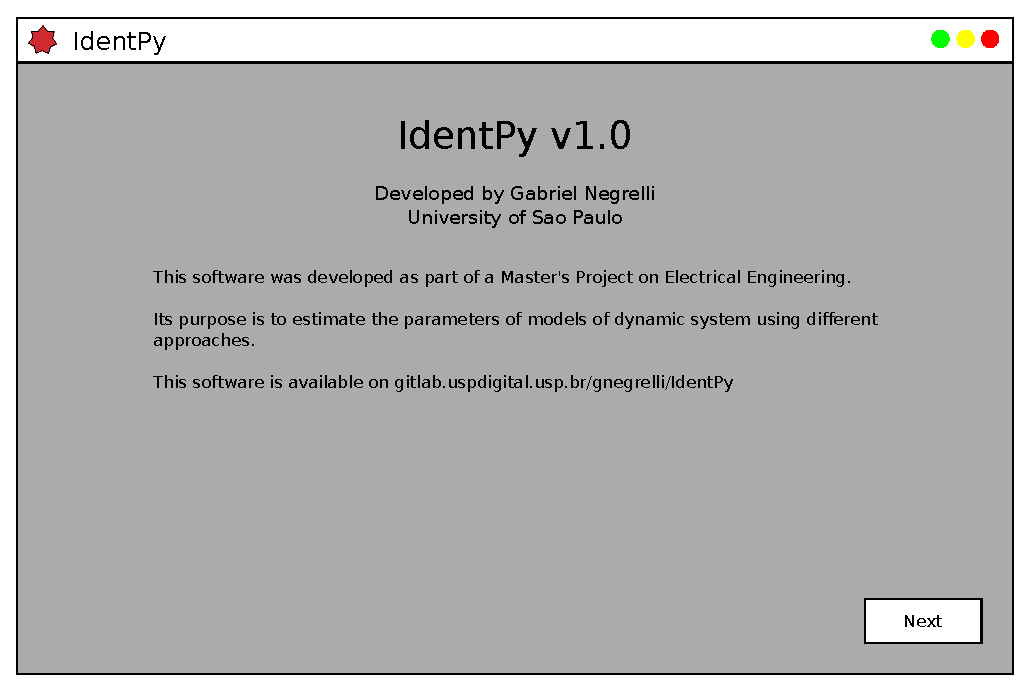
\includegraphics[scale=.5]{Images/Software_init_pg.eps}
	\end{center}
	\label{fig: initial_page}
\end{figure}

Next, the user will choose, from a list, which mathematical model will be estimated, as depicted in Figure \ref{fig: model_selection}. In this view, the user will also select the file containing the measured data and provide the initial conditions of the model. After that, the user will be able to select two estimation methods from the list of available methods, as displayed in Figure \ref{fig: method_selection}.

\begin{figure}[h]
	\caption{Representation of model selection view}
	\begin{center}
		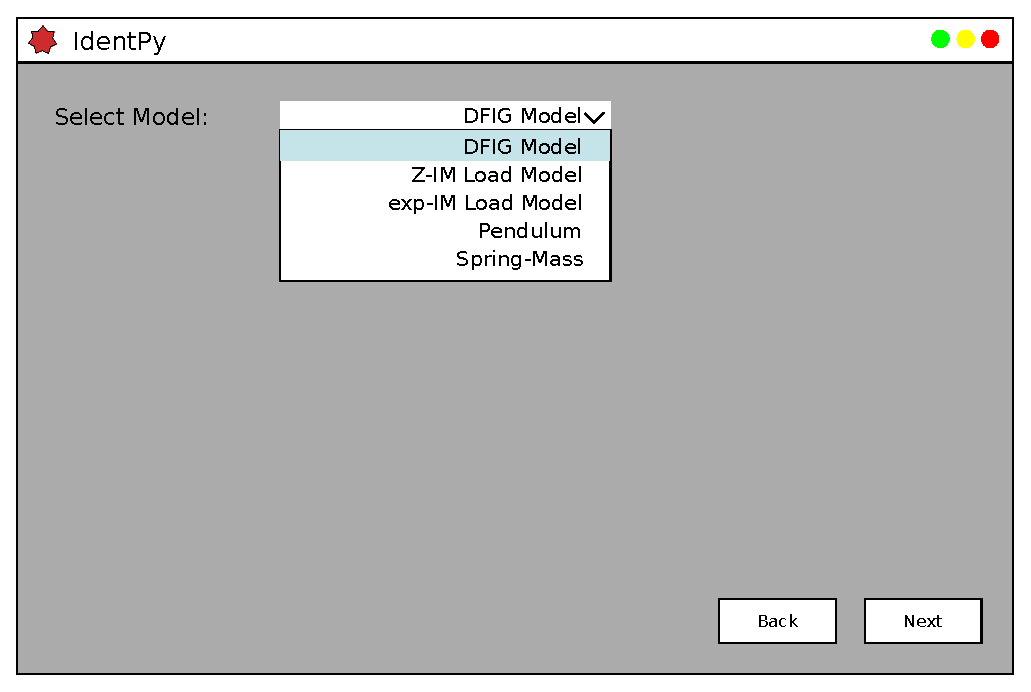
\includegraphics[scale=.5]{Images/Software_pg1.eps}
	\end{center}
	\label{fig: model_selection}
\end{figure}

\begin{figure}[h]
	\caption{Representation of method selection view}
	\begin{center}
		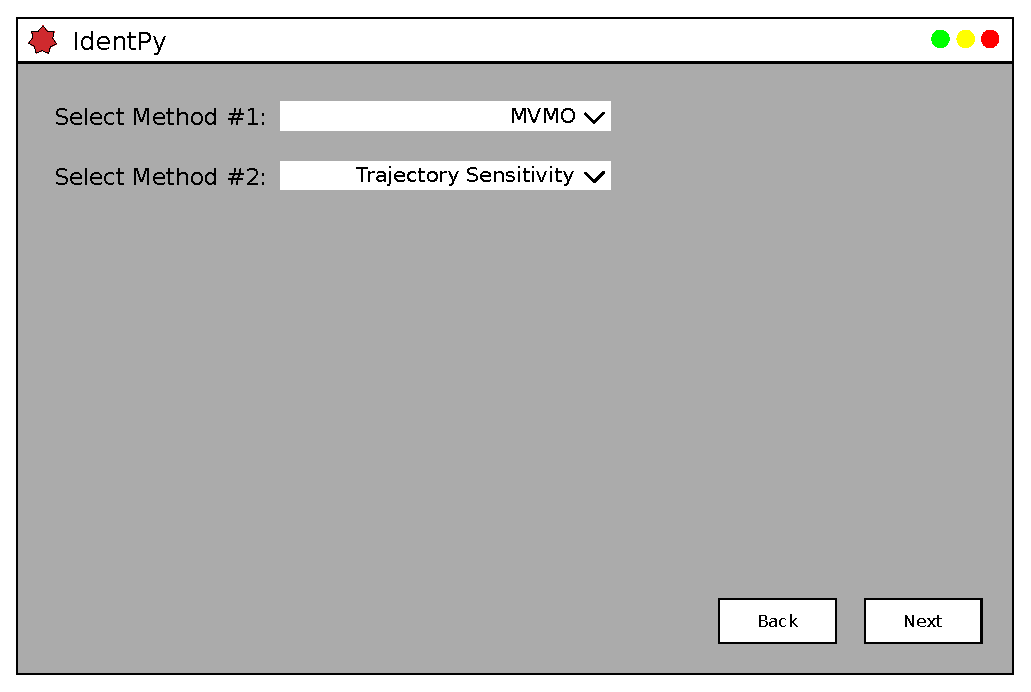
\includegraphics[scale=.5]{Images/Software_pg2.eps}
	\end{center}
	\label{fig: method_selection}
\end{figure}

The configuration of the chosen methods is done on the following windows. Each method has its own configuration page and the view created for setting up MVMO and TS are shown in Figures \ref{fig: MVMO_page} and \ref{fig: TS_page}, respectively.

\begin{figure}[h]
	\caption{Representation of method setting view}
	\begin{center}
		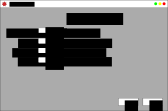
\includegraphics[scale=.5]{Images/Software_pg3.eps}
	\end{center}
	\label{fig: MVMO_page}
\end{figure}

\begin{figure}[h]
	\caption{Representation of file selection view}
	\begin{center}
		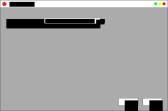
\includegraphics[scale=.5]{Images/Software_pg4.eps}
	\end{center}
	\label{fig: TS_page}
\end{figure}

With all set, the estimation process can now start. A results page with three tabs is displayed to the user while the estimation runs on background. On the first tab, graphs depicting the outputs from the real system and the current solution are shown. The second tab presents the current value of the parameters while the last tab saves a log of the estimation process. Figure \ref{fig: final_pg} presents a view of this page.

\begin{figure}[h]
	\caption{Representation of report view}
	\begin{center}
		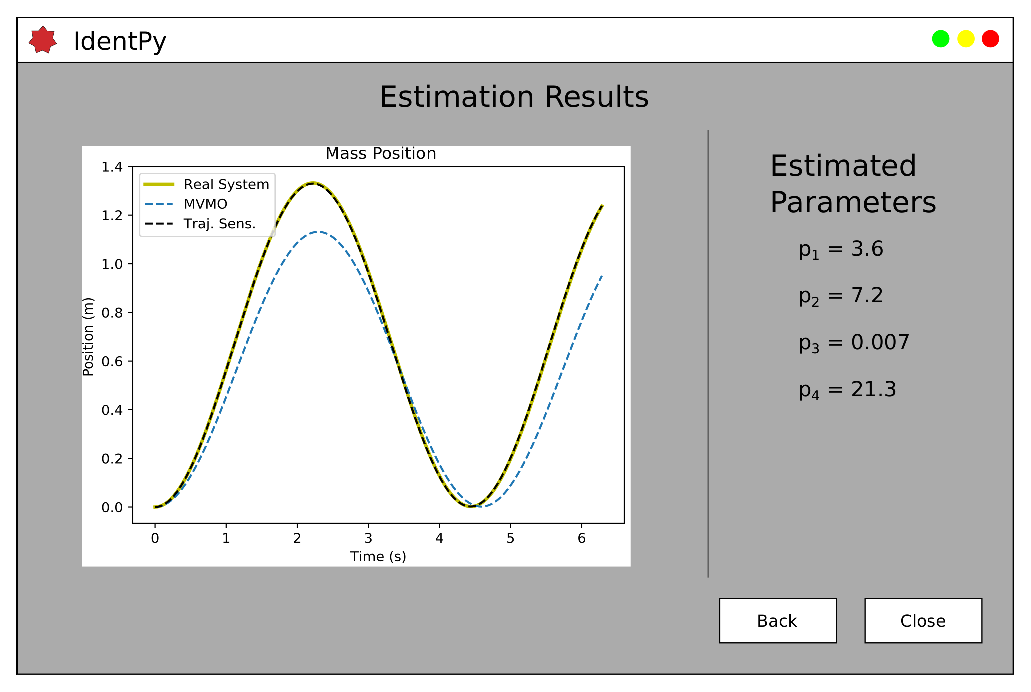
\includegraphics[scale=.5]{Images/Software_final_pg.eps}
	\end{center}
	\label{fig: final_pg}
\end{figure}

As the estimation package evolves, other pages may be included in order to improve the software performance.